%-----------------------------------------------------------------------------%
\chapter{\babDua}
\label{bab:2}
Sebelum memulai pembahasan mendalam mengenai hasil penelitian ini, penting untuk terlebih dahulu meninjau literatur yang relevan. Bab ini akan menyajikan ulasan terhadap teori-teori agar dapat diperoleh landasan teoritis yang kokoh untuk memahami konteks sistem \ir{} dengan \reranker{} berbasis fitur. Sebagai awalan bab, \subbab{}~\ref{subbab:2:Sistem Information Retrieval} menjelaskan salah satu sistem \ir{} yang umum digunakan, yaitu sistem dengan arsitektur \cascaded{}. Kemudian, \subbab{}~\ref{subbab:2:Algoritma Text Matching} membahas mengenai algoritma yang dapat digunakan sebagai fitur dan juga tahap penyaringan atau \ranking{} pertama. Setelah itu, \subbab{}~\ref{subbab:2:Document Encoder} menyampaikan penggunaan \encoder{} dan kaitannya dengan \ir{} sebagai fitur. Terakhir, \subbab{}~\ref{subbab:2:Model Reranker} mendeskripsikan mengenai model \reranker{} yang akan digunakan sebagai tahap \ranking{} kedua.
%-----------------------------------------------------------------------------%





%-----------------------------------------------------------------------------%
\section{Sistem \ir{}}
\label{subbab:2:Sistem Information Retrieval}
Pada dasarnya, \ir{} merujuk pada suatu proses pencarian materi yang sesuai dengan kebutuhan pengguna, umumnya berupa sebuah dokumen, dari himpunan data yang besar atau \corpus{}~\citep{schutze2008introduction}. Selain proses pencarian, \ir{} juga meliputi pembangunan representasi, penyimpanan, dan pengorganisasian dokumen untuk memenuhi kebutuhan tersebut~\citep{baeza1999modern}.

Sistem \ir{} umumnya memiliki arsitektur \cascaded{} dengan lebih dari satu tahap penyaringan dan pengurutan dokumen~\citep{wang2011cascade, nguyen2024captain} yang diilustrasikan pada \gambar{}~\ref{fig:ilustrasi cascade retr}. 
\begin{figure}[!ht]
    \centering
    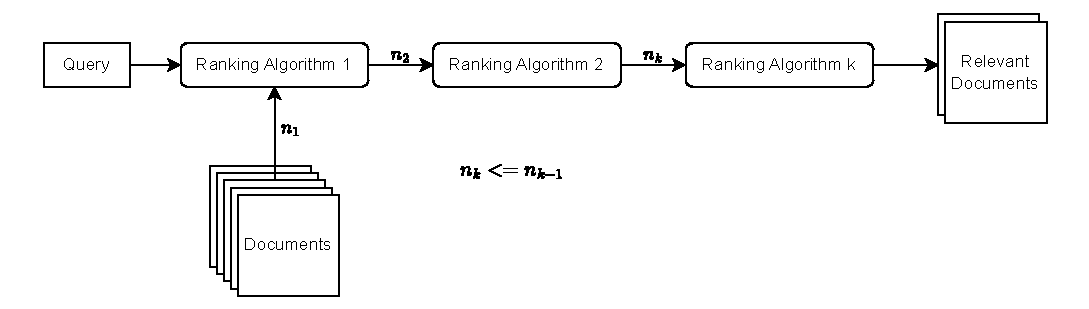
\includegraphics[scale=0.75]{assets/pdfs/CascadeRetrieval.drawio.pdf}
    \caption{Arsitektur \textit{cascaded retrieval}}
    \label{fig:ilustrasi cascade retr}
\end{figure}
Perlu diperhatikan bahwa, untuk setiap tahap \ranking{}, dilakukan penyaringan dan pengurutan dokumen sejumlah \(n_k\) dan dikembalikan dokumen sejumlah \(n_{k+1}\) yang kualitasnya sudah ditingkatkan menggunakan suatu algoritma atau model \ranking{}. Model yang digunakan pada setiap tahap tersebut umumnya dimulai dari suatu algoritma yang efisien seperti algoritma \txt{} \matching{} yang melakukan penyaringan secara \heuristic{}, kemudian diikuti oleh algoritma yang lebih berat secara komputasi seperti model pembelajaran mesin~\citep{zhan2020learning, nguyen2024captain}. Sistem \ir{} dengan arsitektur \cascaded{} inilah yang akan digunakan untuk eksperimen dalam penelitian ini.
%-----------------------------------------------------------------------------%





%-----------------------------------------------------------------------------%
\section{Algoritma \Txt{} \Matching{}}
\label{subbab:2:Algoritma Text Matching}
Algoritma \txt{} \matching{} merupakan algoritma yang umum digunakan sebagai tahap pertama penyaringan dokumen relevan, meskipun kurangnya kemampuan algoritma, seperti \obm{} dan \tfidf{}, dalam menangkap makna semantik dari suatu teks~\citep{zhan2020learning}. Kekurangan algoritma dalam mempertimbangkan makna semantik disebabkan karena perhitungannya yang berfokus pada pencocokan kata. Secara umum, untuk setiap kata \(t\) pada kueri \(q\) dan dokumen \(d\) akan ditentukan bobotnya yang dinotasikan sebagai \(w(t,d)\) dengan \(t\in{}q\). Kemudian, proses \ranking{} menggunakan algoritma tersebut dilakukan dengan mengurutkan skor relevansi \(R\) yang diperoleh menggunakan perhitungan \[
R(q,d)=\sum_{t\in{}q\cap{}d}w(t,d) \, .
\]

\vspace{2mm}
\noindent\textbf{Term Frequency-Inverse Document Frequency (\tfidf{})}. Algoritma ini merupakan salah satu model pembobotan \(w(t,d)\) yang terdiri dari dua bagian. Pertama, bagian \textit{Term Frequency} (TF) sebagai perhitungan frekuensi kemunculan kata pada dokumen yang dinotasikan sebagai 
\[
TF(t,d)=\frac{f(t,d)}{len(d)} \, ,
\]
dengan \(f(t,d)\) adalah jumlah kemunculan kata $t$ pada dokumen $d$; dan $len(d)$ ialah jumlah kata pada dokumen $d$. Sementara itu, bagian kedua dari \tfidf{} adalah \textit{Inverse Document Frequency} (IDF) yang memperhitungkan seberapa umum suatu kata dan mengindikasikan seberapa informatif kata tersebut. Bagian ini memberikan bobot yang lebih tinggi untuk kata-kata yang kemunculannya jarang pada kumpulan dokumen dan bobot yang lebih rendah untuk kata-kata yang umum. Bagian IDF dapat dihitung sebagai
\[
IDF(t)= \log\left(\frac{N}{n}\right) \, ,
\]
dengan $N$ sebagai jumlah dokumen pada koleksi; dan $n$ merupakan jumlah dokumen pada koleksi yang mengandung kata $t$. Kedua bagian tersebut digunakan untuk perhitungan bobot \tfidf{} yang dirumuskan dengan
\[ 
w(t,d)=TF(t,d) \times IDF(t) \, . 
\]

\vspace{2mm}
\noindent\textbf{Okapi \obm{}}. Best Matching 25 atau \obm{} merupakan upaya peningkatan efektivitas algoritma \tfidf{}~\citep{schutze2008introduction}. Pendekatan yang diambil oleh~\citet{robertson1995okapi} untuk meningkatkan efektivitas tersebut adalah dengan perhitungan \textit{eliteness}, penambahan normalisasi panjang dokumen, dan saturasi dari TF~\citep{Robertson2009ThePR}. Bobot untuk algoritma \obm{} dapat dihitung sebagai
\[
w(t,d)=\frac{IDF(t) \times TF(t,d) \times (k_1 + 1)}{TF(t,d) + k_1 (1 - b + b \frac{len(d)}{avgdl})} \, ,
\]
% \[
% BM25(q, d) = \sum^M_{i=1} \frac{IDF(t_{i}) \times TF(t_{i},d) \times (k_1 + 1)}{TF(t_{i},d) + k_1 (1 - b + b \frac{len(d)}{avgdl})} \, ,
% \]
dengan $avgdl$ ialah rata-rata panjang dokumen pada korpus; dan nilai parameter bebas $b$ serta $k_1$.

\vspace{2mm}
\noindent\textbf{Divergence from Randomness} (DFR). Dalam penelitian ini akan digunakan juga model yang menggunakan kerangka DFR~\citep{amati2002probabilistic}. Kerangka tersebut merupakan penggabungan dari dua probabilitas yang dirumuskan sebagai $w(t,d)=(1-P_2(t,d))\cdot(-log_2 P_1(t,d))$ dengan $P_1$ merupakan fungsi probabilitas kemunculan kata $t$ di dokumen $d$ sebagai suatu kebetulan dan $P_2$ adalah probabilitas kemunculan suatu kata $t$ yang ditetapkan sebagai kata penting. Terdapat beberapa model yang menerapkan kerangka ini, salah satunya adalah InL2. Model InL2 menerapkan kerangka DFR dengan Laplace's Law of Succession sebagai model probabilitas $P_2$ yang dapat dihitung menggunakan rumus
\[
P(t,d)=\frac{tf}{tf+1} \, ,
\]
dengan $tf$ merupakan nilai $TF(t,d)$ atau kemunculan kata $t$ pada dokumen $d$. Sementara itu, model \textit{Inverse Document Frequency} digunakan sebagai probabilitas $P_1$ yang dirumuskan secara matematis sebagai
\[
P(t,d)=\left(\frac{n+0.5}{N+1}\right)^{tf} \, ,
\]
dengan $n$ yang merupakan jumlah dokumen dari koleksi sejumlah $N$ yang mengandung kata $t$. Selain dari ketiga model yang telah dijelaskan, yaitu \obm{},\tfidf{}, dan InL2, akan dimanfaatkan beberapa model lain yang dapat ditelusuri secara lebih lanjut pada dokumentasi yang telah disediakan pyterrier\footnote{http://terrier.org/docs/current/javadoc/org/terrier/matching/models/package-summary.html}.
%-----------------------------------------------------------------------------%





%-----------------------------------------------------------------------------%
\section{Document Encoder}
\label{subbab:2:Document Encoder}
Untuk memahami makna semantik dari teks kueri dan dokumen, diperlukan model yang mampu mengekstraksi teks dan menghasilkan representasi semantik dalam bentuk vektor. Dalam konteks ini, model transformer akan digunakan untuk mengekstraksi makna semantik dari teks. Model transformer yang diperkenalkan oleh \citet{vaswani2017attention} merupakan salah satu tipe model \nn{} yang telah merevolusi pemrosesan bahasa alami dan bidang kecerdasan buatan lainnya.

Model transformer tersebut terdiri dari lapisan \encoder{} dan \decoder{} yang divisualisasikan pada~\gambar{}~\ref{fig:ilustrasi transformer}.
\begin{figure}[!ht]
    \centering
    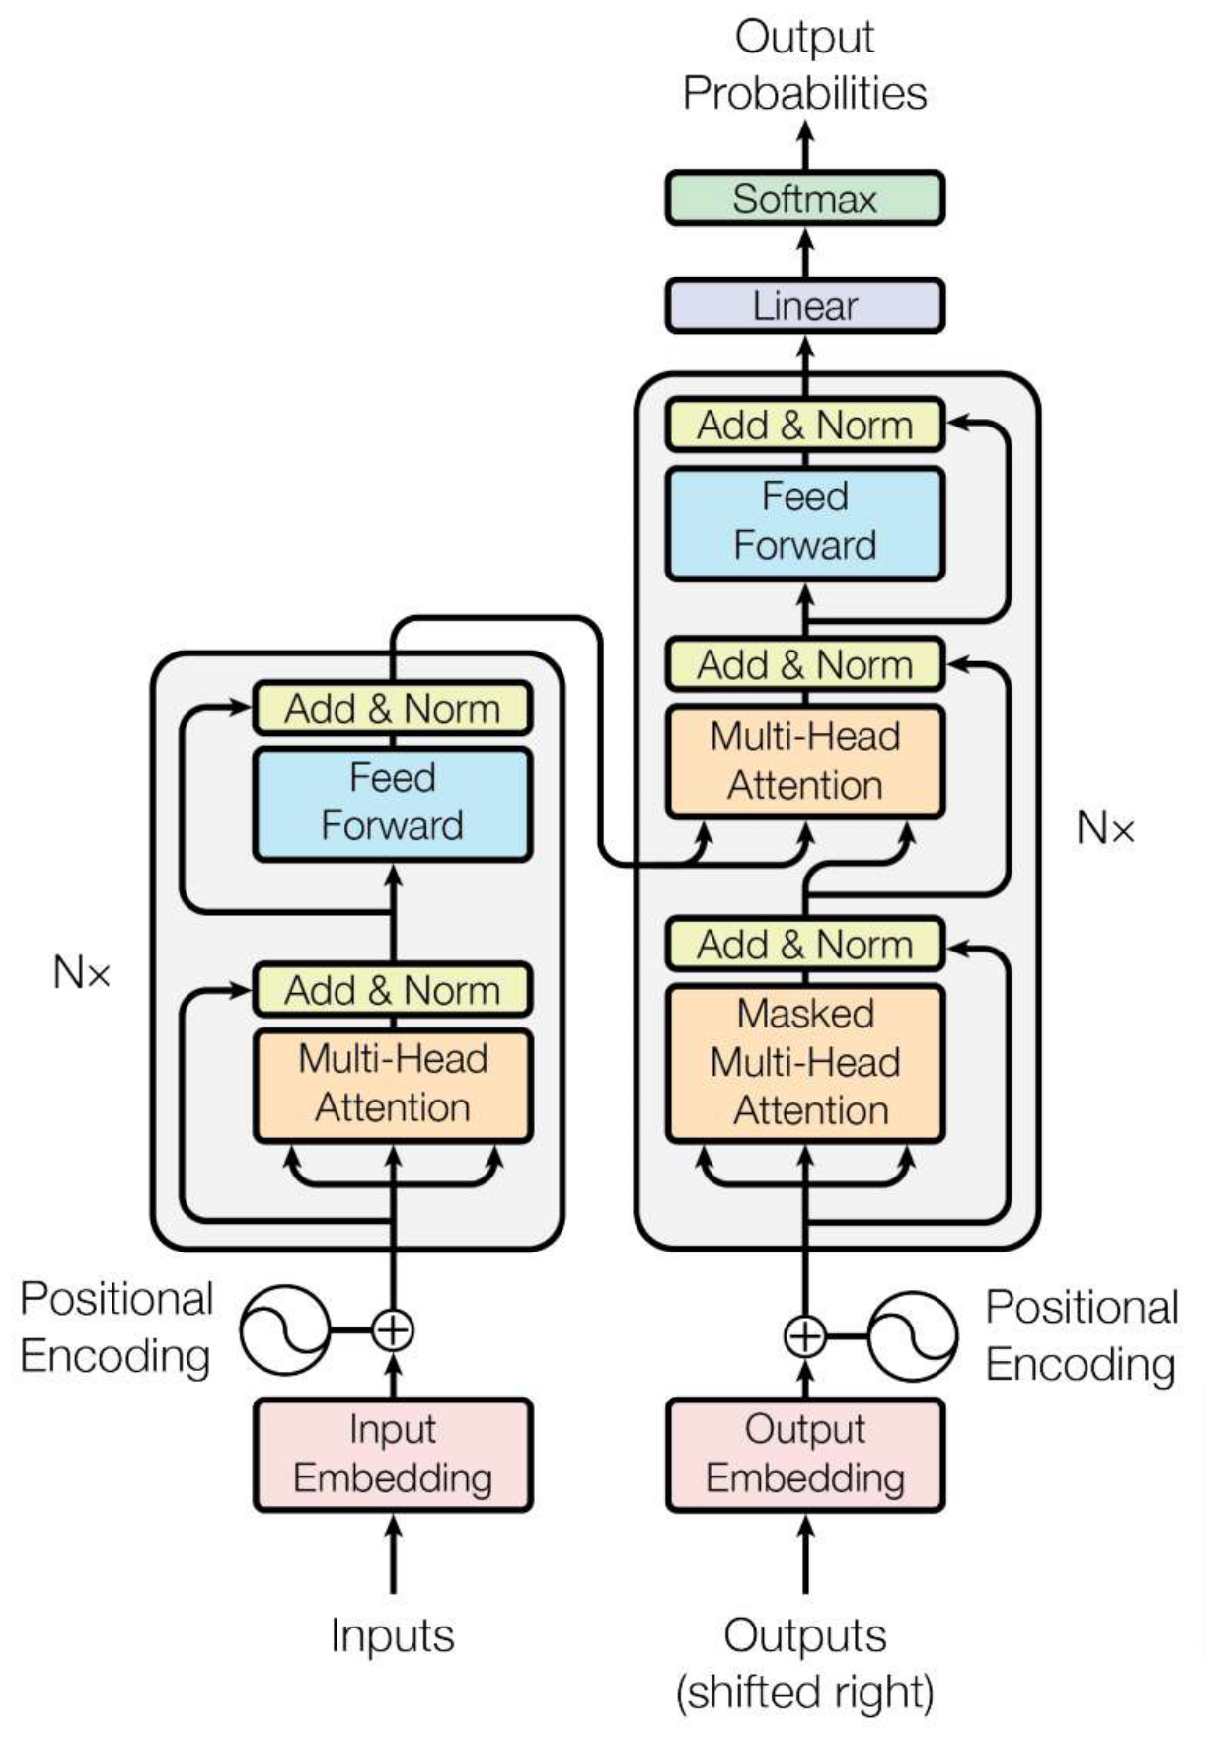
\includegraphics[scale=0.4]{assets/pdfs/transformer_aristektur.pdf}
    \captionsource{Arsitektur transformer}{\citep{vaswani2017attention}}
    \label{fig:ilustrasi transformer}
\end{figure}
Lapisan \encoder{} bekerja dengan mengubah masukan yang berupa teks menjadi vektor yang dapat merepresentasikan makna semantik dari teks tersebut. Kemudian, lapisan \decoder{} digunakan untuk menginterpretasi vektor hasil lapisan \encoder{} dan menghasilkan serangkaian teks sebagai keluaran. Namun, dalam penelitian ini, karena model transformer hanya diperlukan untuk melakukan ekstraksi hasil vektor representasi teks, maka hanya akan menggunakan lapisan \encoder{} dalam eksperimen.

Pengembangan utama dari arsitektur transformer dibandingkan dengan model-model \nn{} lainnya adalah mekanisme \textit{self-attention} yang memungkinkan model untuk memperhitungkan pentingnya setiap \textit{token} relatif satu sama lain di dalam kalimat. Mekanisme ini memungkinkan model untuk menangkap dependensi atau hubungan tanpa dibatasi oleh jarak antar urutan masukan, suatu hal yang terbatas pada model seperti RNN (Recurrent Neural Network) maupun CNN (Convolutional Neural Network). Namun, karena mekanisme \textit{self-attention} yang tidak mengandalkan alur seperti RNN, maka model transformer perlu mendapatkan informasi tambahan terkait posisi dari \textit{token} dalam urutan. Oleh karena itu, \citeauthor{vaswani2017attention} mengusulkan \textit{positional encoding} agar transformer dapat memanfaatkan informasi dari alur \textit{token}. Selain itu, perlu diperhatikan bahwa untuk setiap \textit{sub-layer} dari \encoder{} dan \decoder{} diimplementasikan \textit{feed-forward network} dan \textit{layer} normalisasi untuk stabilitas dan efisiensi pelatihan.

\vspace{2mm}
\noindent\textbf{\lbert{} (\bert{}).}
\lbert{} (\bert{}) adalah arsitektur yang memanfaatkan bagian \encoder{} dari transformer yang dirancang oleh Google untuk memahami konteks atau makna semantik dari kata di dalam suatu kalimat dengan pendekatan pemrosesan secara \textit{bidirectional}~\citep{devlin2018bert}. Dengan pendekatan ini, \bert{} dapat menangkap hubungan dan konteks antara kata-kata dalam kalimat, baik sebelum atau sesudah kata tertentu. Hal tersebut memungkinkan \bert{} untuk mendapatkan pemahaman yang lebih baik tentang makna kata dalam konteks kalimat yang lebih luas.

Model \bert{} memiliki arsitektur yang memanfaatkan 12 \encoder{} yang bernamakan \textit{hidden layer} seperti yang ditunjukkan pada \gambar{}~\ref{fig:ilustrasi bert}.
\begin{figure}[!ht]
    \centering
    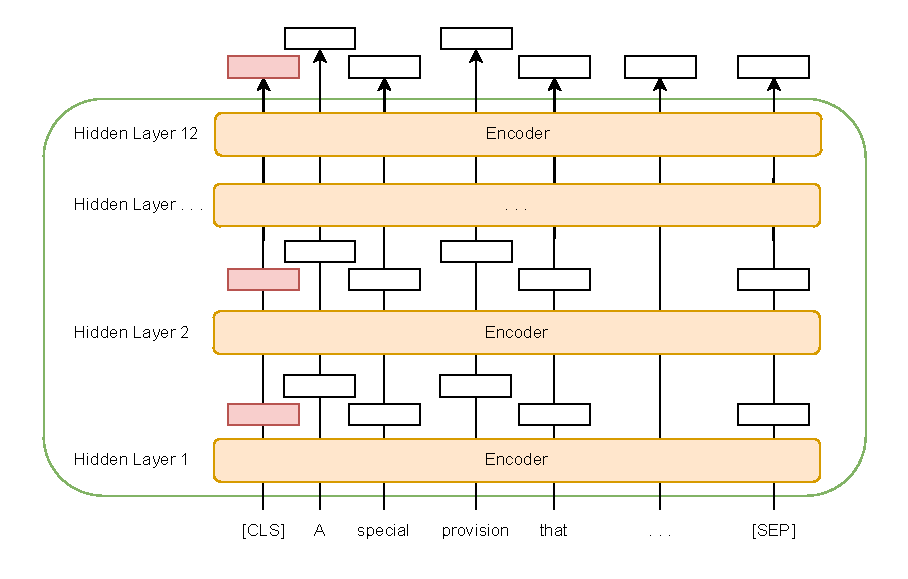
\includegraphics[scale=0.75]{assets/pdfs/IlustrasiBERT.drawio.pdf}
    \caption{Arsitektur model \bert{}}
    \label{fig:ilustrasi bert}
\end{figure}
Perhatikan bahwa masukan untuk model \bert{} merupakan kalimat yang telah dikonversi menjadi \textit{token} dengan tambahan beberapa \textit{token} khusus yang menandakan awal dan akhir kalimat, yaitu ``[CLS]'' dan ``SEP''. Kemudian masukan tersebut akan melewati beberapa pemrosesan oleh \encoder{} sejumlah 12 kali yang dapat dinotasikan sebagai
\[
HS_{n}=ENC_{n}(HS_{n-1}) \, ,
\]
dengan $HS_{n}$ merupakan \hs{} atau keluaran dari \encoder{} pada \textit{layer} ke-$n$; dan $ENC_{n}$ merupakan \encoder{} atau \textit{hidden layer} ke-$n$.

\vspace{2mm}
\noindent\textbf{\ttttt{} (\tfive{}).}
\ttttt{} adalah suatu tipe model yang menerapkan arsitektur transformer. Model ini dirancang untuk berbagai tugas pemrosesan bahasa alami yang secara spesifik dilatih menggunakan kerangka kerja \txt{}-to-\txt{}~\citep{raffel2020exploring}. Berbeda dengan model lain yang dilatih untuk tugas tertentu, model \tfive{} dapat dilatih menggunakan satu tujuan, yaitu mengonversi teks masukan menjadi teks keluaran. Arsitektur \tfive{} serupa dengan \bert{} dengan fokus pada penelitian ini khusus pada bagian \encoder{} dari \tfive{} yang dapat dilihat pada \gambar{}~\ref{fig:ilustrasi t5}
\begin{figure}[!ht]
    \centering
    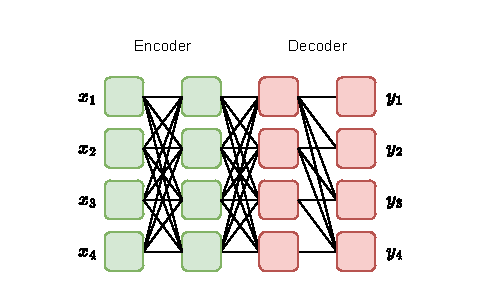
\includegraphics[scale=1.5]{assets/pdfs/t5 structure.drawio.pdf}
    \caption{Arsitektur model \tfive{}}
    \label{fig:ilustrasi t5}
\end{figure}
%-----------------------------------------------------------------------------%





%-----------------------------------------------------------------------------%
\section{Model \Reranker{}}
\label{subbab:2:Model Reranker}
Seperti yang telah dijelaskan pada \bab~\ref{subbab:2:Sistem Information Retrieval}, sebagai suatu upaya perbaikan pada tahap \ranking{} pertama dalam sistem \ir{} dengan arsitektur \cascaded{}, terdapat suatu tahap tambahan, yaitu \reranking{}. Tahap \reranking{} ini, umumnya memerlukan kemampuan komputasi yang lebih tinggi dibanding hanya menggunakan suatu algoritma \txt{} \matching{}~\citep{zhan2020learning}. Salah satu model \reranker{} yang umum digunakan untuk tugas \ranking{} adalah \lambdamart{}, model yang akan digunakan sebagai tahap \ranking{} kedua pada penelitian ini.

\subsection{\ranknet{}}
\label{subbab:2:RankNet}
\ranknet{}~\citep{burges2010ranknet} adalah sebuah model pembelajaran mesin yang dapat  yang secara spesifik dirancang untuk \ltr{} yang digunakan umumnya untuk tugas pemeringkatan seperti \ir{}. Model tersebut dapat diimplementasikan menggunakan model \nn{} maupun model \textit{boosted tree} yang menerima suatu vektor $v \in{} \mathbb{R}^n$ dan mengembalikan nilai riil $f(v)$. Diberikan suatu kueri pada pelatihan, \ranknet{} akan terlebih dahulu menghitung skor untuk setiap dokumen dengan $s_{i}=f(v_{i})$, kemudian melakukan komputasi probabilitas $P_{ij}$ yang merupakan kemungkinan dokumen $i$ yang seharusnya ditempatkan pada posisi yang lebih tinggi dibandingkan $j$. Probabilitas tersebut dihitung menggunakan
\[
P_{ij} = \frac{1}{1+e^{-(s_i-s_j)}} \, .
\]

Setelah melakukan komputasi probabilitas untuk setiap pasangan kueri dan dokumen, akan dihitung \textit{cross-entropy loss} $L$ yang didefinisikan sebagai
\[
L=-\bar{P_{ij}}\log{P_{ij}}-(1-\bar{P_{ij}})\log(1-P_{ij}) \, ,
\]
yang kemudian disederhanakan menjadi 
\begin{align*}
L=\frac{(1-S_{ij})}{2}\sigma{}(s_i-s_j)+\log{}(1+e^{-\sigma{}(s_i-s_j)}) \, ,
\end{align*}
dengan $S_{ij}\in{}\{0,\pm{}1\}$ merupakan relevansi yang telah diketahui untuk dokumen yang bernilai 1 ketika dokumen $i$ memiliki label lebih relevan dibanding dokumen $j$, bernilai -1 sebaliknya, dan bernilai 0 ketika label kedua dokumen sama.

\subsection{\lambdarank{}}
\label{subbab:2:LambdaRank}
Model ini merupakan upaya pengembangan \ranknet{} karena saat perancangannya, terdapat asumsi bahwa perhitungan skor masing-masing dokumen merupakan skor yang ideal~\citep{burges2010ranknet}. Salah satu perbedaan \lambdarank{} dan \ranknet{} tidak dibutuhkannya perhitungan \textit{loss} melainkan hanya diperlukan gradien dari nilai tersebut. Gradien tersebut dihitung menggunakan
\[
\lambda_{ij}=\frac{\delta{}L(s_i-s_j)}{\delta{}s_i}=\frac{-\sigma{}}{1+e^{\sigma{}(s_i-s_j)}}|\Delta{}NDCG| \, ,
\]
dengan nilai $NDCG$ sebagai
\begin{align*}
DCG@k&\equiv{}\sum^k_{i=1} \frac{2^{l_i}-1}{\log(1+i)} \, ,\\
NDCG@k&\equiv{}\frac{DCG@k}{maxDCG@k} \, ,
\end{align*}
dengan $k$ merupakan nilai \cutoff{}; dan $l_i$ adalah label dari dokumen $i$. Setelah itu, model melakukan pembaruan bobot menggunakan akumulasi dari gradien tersebut.

\subsection{\lambdamart{}}
\label{subbab:2:LambdaMART}
\lambdamart{} adalah gabungan dari dua buah komponen, yaitu \lambdarank{} dan MART. Multiple Additive Regression Trees (MART) adalah suatu model \textit{ensemble} yang terdiri dari \textit{boosted decision trees}. Dalam model MART, setiap struktur \textit{tree} akan mencoba untuk memperbaiki hasil struktur \textit{tree} sebelumnya untuk meningkatkan kinerja secara menyeluruh. 

Berbeda dengan \lambdarank{} yang memperbarui semua bobot setelah setiap kueri diperiksa. Sebaliknya, dalam \lambdamart{}, keputusan (pemisahan pada \textit{node}) dihitung menggunakan semua data yang berada di \textit{node} tersebut, sehingga \lambdamart{} hanya memperbarui beberapa parameter pada satu waktu. Hal ini berarti LambdaMART dapat memilih pemisahan dan nilai \textit{leaf} yang mungkin menurunkan efektivitas untuk beberapa kueri, asalkan efektivitas keseluruhan meningkat~\citep{burges2010ranknet}.
%-----------------------------------------------------------------------------%

% Dalam penelitian ini, akan dikaji beberapa algoritma yang umum digunakan dalam konteks \ir{} untuk dokumen legal~\citep{goebel2023summary}.